\documentclass{article}
\usepackage{amsmath, amssymb, amsthm, pgfplots}
\pgfplotsset{compat=1.8}

% Definir estilos
\theoremstyle{definition} 
\newtheorem{problem}{Problema} 
\newtheorem*{solution}{Solución} 

\begin{document}

\title{Ejercicios del Apartado 2.3. \\ (p. 62)}
\author{Simmons, George F. \\ \textit{Calculus with Analytic Geometry. 2nd ed.}}
\date{Febrero de 2025}
\maketitle

\begin{problem}
Utiliza la regla de los tres pasos para demostrar que si \( f(x) = ax^2 + bx + c \), entonces \( f'(x) = 2ax + b \).
\end{problem}

\medskip

\begin{solution}
La regla de los tres pasos consiste en:
    \begin{enumerate}
        \item Calcular \( f(x+\Delta x)-f(x)\)
        \item Dividir el resultado por \( \Delta x\)
        \item Calcularlo el \( \lim_{\Delta x \to 0} \) de lo obtenido
    \end{enumerate}
En este caso:
    \begin{align*}
        f(x+\Delta x) - f(x) &= a(x+ \Delta x)^2+b(x+\Delta x)+c-(ax^2+bx+c) \\
        &= a(x^2+2x\Delta x+(\Delta x^2))+bx+b\Delta x+c-ax^2-bx-c \\
        &= ax^2+2ax\Delta x+a\Delta x^2+bx+b\Delta x+c-ax^2-bx-c \\
        &=2ax\Delta x+a\Delta x^2+b\Delta x
    \end{align*}
Dividimos el resultado por \( \Delta x \):
    \begin{align*}
        &= \frac{2ax\Delta x+a\Delta x^2+b\Delta x}{\Delta x} \\
        &= 2ax + a \Delta x + b
    \end{align*}
Calculamos el \( \lim_{\Delta x \to 0} \) del resultado:
    \begin{align*}
        \lim_{\Delta x \to 0} (2ax + a \Delta x + b) &= 2ax+b
    \end{align*}
\end{solution}

\bigskip

\begin{problem}
Usa la regla general del Problema 1 para escribir las derivadas indicadas en los Problemas 2-16.
\begin{enumerate}
    \item \( f(x) = 5x - 3 \); encuentra \( f'(x) \).
    \item \( g(x) = 50 - 8x^2 \); encuentra \( g'(x) \).
    \item \( h(x) = x(50 - x) \); encuentra \( h'(x) \).
    \item \( F(x) = 20 - 72x \); encuentra \( F'(x) \).
    \item \( G(x) = 3x^2 + 5x - 7 \); encuentra \( G'(x) \).
    \item \( H(x) = 5 - 10x + 15x^2 \); encuentra \( H'(x) \).
    \item \( y = 5x^2 - 9x + 15 \); encuentra \( \frac{dy}{dx} \).
    \item \( x = 3y^2 + 7y - 6 \); encuentra \( \frac{dx}{dy} \).
    \item \( u = 7t^2 - 11t + 109 \); encuentra \( \frac{du}{dt} \).
    \item \( v = 7x(500 - x) \); encuentra \( \frac{dv}{dx} \).
    \item \( w = -7z^2 + 22z - 71 \); encuentra \( \frac{dw}{dz} \).
    \item \( f(x) = 5x(x + 5) \); encuentra \( f'(x) \).
    \item \( y = 5x - (x/10) \); encuentra \( \frac{dy}{dx} \).
    \item \( g(x) = 3 - (4x + 5)^2 \); encuentra \( g'(x) \).
    \item \( h(x) = (3x - 2)^2 - 5x \); encuentra \( h'(x) \).
\end{enumerate}
\end{problem}

\medskip

\begin{solution}

\textbf{Inciso 1}:

    \begin{align*}
        f(x+\Delta x) - f(x) &= 5(x+\Delta x)-3-(5x-3) \\
        &= 5x+5\Delta x-3-5x+3 \\
        &= 5\Delta x
    \end{align*}

    \begin{align*}
        \frac{5\Delta x}{\Delta x} &= 5
    \end{align*}

    \begin{align*}
        \lim_{\Delta x \to 0} (5) &= 5
    \end{align*}

\textbf{Inciso 2}:

    \begin{align*}
        g(x+\Delta x) - g(x) &= 50-8(x+\Delta x)^2-(50-8x^2) \\
        &= 50-8(x^2+2x\Delta x+(\Delta x)^2)-50+8x^2 \\
        &= 50-8x^2-16x\Delta x-8(\Delta x)^2-50+8x^2 \\
        &= -16x\Delta x-8(\Delta x)^2
    \end{align*}

    \begin{align*}
        \frac{-16x\Delta x-8(\Delta x)^2}{\Delta x} &= -16x-8\Delta x
    \end{align*}

    \begin{align*}
        \lim_{\Delta x \to 0} (-16x-8\Delta x) &= -16x
    \end{align*}

\textbf{Inciso 3}:

    \begin{align*}
        h(x) &= x(50-x) \\
        &= -x^2+50x
    \end{align*}

    \begin{align*}
        h(x+\Delta x) - h(x) &= -(x+\Delta x)^2+50(x+\Delta x)-(-x^2+50x) \\
        &= -(x^2+2x\Delta x+(\Delta x)^2)+50x+50\Delta x+x^2-50x \\
        &= -x^2-2x\Delta x-(\Delta x)^2+50x+50\Delta x+x^2-50x \\
        &= -2x\Delta x-(\Delta x)^2+50\Delta x
    \end{align*}

    \begin{align*}
        \frac{-2x\Delta x-(\Delta x)^2+50\Delta x}{\Delta x} &= -2x-\Delta x+50
    \end{align*}

    \begin{align*}
        \lim_{\Delta x \to 0} (-2x-\Delta x+50) &= -2x+50
    \end{align*}

\textbf{Inciso 4}:

    \begin{align*}
        F(x+\Delta x) - F(x) &= 20-72(x+\Delta x)-(20-72x) \\
        &= 20-72x-72\Delta x-20+72x \\
        &= -72\Delta x
    \end{align*}

    \begin{align*}
        \frac{-72\Delta x}{\Delta x} &= -72
    \end{align*}

    \begin{align*}
        \lim_{\Delta x \to 0} (-72) &= -72
    \end{align*}

\textbf{Inciso 5}:

    \begin{align*}
        G(x+\Delta x) - G(x) &= 3(x+\Delta x)^2+5(x+\Delta x)-7-(3x^2+5x-7) \\
        &= 3(x^2+2x\Delta x+(\Delta x)^2)+5x+5\Delta x-7-3x^2-5x+7 \\
        &= 3x^2+6x\Delta x+3(\Delta x)^2+5x+5\Delta x-7-3x^2-5x+7 \\
        &= 6x\Delta x+3(\Delta x)^2+5\Delta x
    \end{align*}

    \begin{align*}
        \frac{6x\Delta x+3(\Delta x)^2+5\Delta x}{\Delta x} &= \frac{\Delta x(6x+3\Delta x+5)}{\Delta x} \\
        &= 6x+3\Delta x+5
    \end{align*}

    \begin{align*}
        \lim_{\Delta x \to 0} (6x+3\Delta x+5) &= 6x+5
    \end{align*}

\textbf{Inciso 6}:

    \begin{align*}
        H(x+\Delta x) - H(x) &= 5-10(x+\Delta x)+15(x+\Delta x)^2-(5-10x+15x^2) \\
        &= 5-10x-10\Delta x+15(x^2+2x\Delta x+(\Delta x)^2-5+10x-15x^2 \\
        &= 5-10x-10\Delta x+15x^2+30x\Delta x+15(\Delta x)^2-5+10x-15x^2 \\
        &= -10\Delta x+30x\Delta x+15(\Delta x)^2
    \end{align*}

    \begin{align*}
        \frac{-10\Delta x+30x\Delta x+15(\Delta x)^2}{\Delta x} &= \frac{\Delta x(-10+30x+15\Delta x)}{\Delta x} \\
        &= -10+30x+15\Delta x
    \end{align*}

    \begin{align*}
        \lim_{\Delta x \to 0} (-10+30x+15\Delta x) &= -10+30x
    \end{align*}

\textbf{Inciso 7}:

    \begin{align*}
        y(x+\Delta x) - y(x) &= 5(x+\Delta x)^2-9(x+\Delta x)+15-(5x^2-9x+15) \\
        &= 5(x^2+2x\Delta x+(\Delta x)^2)-9x-9\Delta x+15-5x^2+9x-15 \\
        &= 5x^2+10x\Delta x+5(\Delta x)^2-9x-9\Delta x+15-5x^2+9x-15 \\
        &= 10x\Delta x+5(\Delta x)^2-9\Delta x
    \end{align*}

    \begin{align*}
        \frac{10x\Delta x+5(\Delta x)^2-9\Delta x}{\Delta x} &= \frac{\Delta x(10x+5\Delta x-9)}{\Delta x} \\
        &= 10x+5\Delta x-9
    \end{align*}

    \begin{align*}
        \lim_{\Delta x \to 0} (10x+5\Delta x-9) &= 10x-9
    \end{align*}

\textbf{Inciso 8}:

    \begin{align*}
        x(y+\Delta y) - x(y) &= 3(y+\Delta y)^2+7(y+\Delta y)-6-(3y^2+7y-6) \\
        &= 3(y^2+2y\Delta y+(\Delta y)^2)+7y+7\Delta y-6-3y^2-7y+6 \\
        &= 3y^2+6y\Delta y+3(\Delta y)^2+7y+7\Delta y-6-3y^2-7y+6 \\
        &= 6y\Delta y+3(\Delta y)^2+7\Delta y
    \end{align*}

    \begin{align*}
        \frac{6y\Delta y+3(\Delta y)^2+7\Delta y}{\Delta y} &= \frac{\Delta y(6y+3\Delta y+7)}{\Delta y} \\
        &= 6y+3\Delta y+7
    \end{align*}

    \begin{align*}
        \lim_{\Delta y \to 0} (6y+3\Delta y+7) &= 6y+7
    \end{align*}

\textbf{Inciso 9}:

    \begin{align*}
        u(t+\Delta t) - u(t) &= 7(t+\Delta t)^2-11(t+\Delta t)+109 - (7t^2-11t+109) \\
        &= 7(t^2+2t\Delta t+(\Delta t)^2)-11t-11\Delta t+109-7t^2+11t-109 \\
        &= 7t^2+14t\Delta t+7(\Delta t)^2-11t-11\Delta t+109-7t^2+11t-109 \\
        &= 14t\Delta t+7(\Delta t)^2-11\Delta t
    \end{align*}

    \begin{align*}
        \frac{14t\Delta t+7(\Delta t)^2-11\Delta t}{\Delta t} &= \frac{\Delta t(14t+7\Delta t-11)}{\Delta t}
    \end{align*}

    \begin{align*}
        \lim_{\Delta t \to 0} (14t+7\Delta t-11) &= 14t-11
    \end{align*}

\textbf{Inciso 10}:

    \begin{align*}
        v(x+\Delta x) - v(x) &= 7(x+\Delta x)(500-(x+\Delta x))-7x(500-x) \\
        &= (7x+7\Delta x)(500-x-\Delta x)-3500x+7x^2 \\
        &= 3500x - 7x^2 - 7x\Delta x + 3500\Delta x - 7x\Delta x-7(\Delta x)^2-3500x + 7x^2 \\
        &= -2(7x\Delta x)+3500\Delta x - 7(\Delta x)^2
    \end{align*}

    \begin{align*}
        \frac{-2(7x\Delta x)+3500\Delta x - 7(\Delta x)^2}{\Delta x} &= \frac{\Delta x(-14x+3500-7\Delta x)}{\Delta x} \\
        &= -14x+3500-7\Delta x
    \end{align*}

    \begin{align*}
        \lim_{\Delta x \to 0} (-14x+3500-7\Delta x) &= -14x+3500
    \end{align*}

\textbf{Inciso 11}:

    \begin{align*}
        w(z+\Delta z) - w(z) &= -7(z+\Delta z)^2+22(z+\Delta z)-71-(-7z^2+22z-71) \\
        &= -7(z^2+2z\Delta z+(\Delta z)^2)+22z+22\Delta z-71+7z^2-22z+71 \\
        &= -7z^2-14z\Delta z-7(\Delta z)^2+22z+22\Delta z-71+7z^2-22z+71 \\
        &= -14z\Delta z-7(\Delta z)^2+22\Delta z
    \end{align*}

    \begin{align*}
        \frac{-14z\Delta z-7(\Delta z)^2+22\Delta z}{\Delta z} &= \frac{\Delta z(-14z-7\Delta z+22)}{\Delta z} \\
        &= -14z-7\Delta z+22
    \end{align*}

    \begin{align*}
        \lim_{\Delta z \to 0} (-14z-7\Delta z+22) &= -14z+22
    \end{align*}

\textbf{Inciso 12}:

    \begin{align*}
        f(x+\Delta x) - f(x) &= 5(x+\Delta x)((x+\Delta x)+5)-(5x(x+5)) \\
        &= 5(x+\Delta x)(x+\Delta x+5)-(5x^2+25x) \\
        &= 5(x^2+x\Delta x+5x+x\Delta x+(\Delta x)^2+5\Delta x)-5x^2-25x \\
        &= 5x^2+5x\Delta x+25x+5x\Delta x+5(\Delta x)^2+25\Delta x-5x^2-25x \\
        &= 10x\Delta x+5(\Delta x)^2+25\Delta x
    \end{align*}

    \begin{align*}
        \frac{10x\Delta x+5(\Delta x)^2+25\Delta x}{\Delta x} &= \frac{\Delta x(10x+5\Delta x+25)}{\Delta x} \\
        &= 10x+5\Delta x+25
    \end{align*}

    \begin{align*}
        \lim_{\Delta x \to 0} (10x+5\Delta x+25) &= 10x+25
    \end{align*}

\textbf{Inciso 13}:

    \begin{align*}
        y &= 5x-(\frac{x}{10}) \\
        y &= \frac{50x-x}{10} \\
        y &= \frac{49x}{10}
    \end{align*}

    \begin{align*}
        y(x+\Delta x)-y(x) &= \frac{49(x+\Delta x)}{10} - \frac{49x}{10} \\
        &= \frac{49x+49\Delta x - 49x}{10} \\
        &= \frac{49\Delta x}{10}
    \end{align*}

    \begin{align*}
        &= \frac{\frac{49\Delta x}{10}}{\Delta x} \\
        &= \frac{49}{10}
    \end{align*}

    \begin{align*}
        \lim_{\Delta x \to 0} (\frac{49}{10}) &= \frac{49}{10}
    \end{align*}

\textbf{Inciso 14}:

    \begin{align*}
        g(x+\Delta x)-g(x) &= 3-(4(x+\Delta x)+5)^2-(3-(4x+5)^2) \\
        &= 3-((4(x+\Delta x))^2+40(x+\Delta x)+25)-(3-(16x^2+40x+25)) \\
        &= 3-(16x^2+32x\Delta x+16(\Delta x)^2+40x+40\Delta x+25)-3+16x^2+40x+25 \\
        &= 3-16x^2-32x\Delta x-16(\Delta x)^2-40x-40\Delta x-25-3+16x^2+40x+25 \\
        &= -32x\Delta x-16(\Delta x)^2-40\Delta x
    \end{align*}

    \begin{align*}
        &= \frac{-32x\Delta x-16(\Delta x)^2-40\Delta x}{\Delta x} \\
        &= \frac{\Delta x(-32x-16\Delta x-40)}{\Delta x} \\
        &= -32x-16\Delta x-40
    \end{align*}

    \begin{align*}
        \lim_{\Delta x \to 0} (-32x-16\Delta x-40) &= -32x-40
    \end{align*}

\textbf{Inciso 15}:

    \begin{align*}
        h(x+\Delta x)-h(x) &= (3(x+\Delta x)-2)^2-5(x+\Delta x) - ((3x-2)^2-5x) \\
        &= ((3x+3\Delta x)-2)^2-5x-5\Delta x - ((3x-2)^2-5x) \\
        &= (3x+3\Delta x)^2-4(3x+3\Delta x)+4-5x-5\Delta x - ((3x-2)^2-5x) \\
        &= 9x^2+18x\Delta x+9(\Delta x)^2-12x-12\Delta x+4-5x-5\Delta x - ((9x^2-12x+4)-5x) \\
        &= 9x^2+18x\Delta x+9(\Delta x)^2-12x-12\Delta x+4-5x-5\Delta x -9x^2+12x-4+5x \\
        &= 18x\Delta x+9(\Delta x)^2-17\Delta x
    \end{align*}

    \begin{align*}
        &= \frac{18x\Delta x+9(\Delta x)^2-17\Delta x}{\Delta x} \\
        &= \frac{\Delta x(18x+9\Delta x-17)}{\Delta x} \\
        &= 18x+9\Delta x-17
    \end{align*}

    \begin{align*}
        \lim_{\Delta x \to 0} (18x+9\Delta x-17) &= 18x-17
    \end{align*}

\end{solution}

\bigskip

\begin{problem}
Encuentra todos los puntos de la curva \( y = f(x) \) donde la tangente es horizontal.
\begin{enumerate}
    \item \( y = 6 - x^2 \).
    \item \( y = 6x - x^2 \).
    \item \( y = x^2 - 6x + 9 \).
    \item \( y = x^2 + x - 5 \).
    \item \( y = x(20 - x) \).
    \item \( y = x - (x/20) \).
\end{enumerate}
\end{problem}

\medskip

\begin{solution}

Para encontrar los puntos en donde la tangente es horizontal:
\begin{enumerate}
    \item Calculamos la derivada de la función.
    \item Igualamos la derivada a \( 0 \).
    \item Resolvemos esa derivada para \( x \).
    \item Evaluamos la función en \( y \) para esa \( x \).
\end{enumerate}

\textbf{Inciso 1:} 

Calculamos la derivada de la función:

    \[
        y = 6 - x^2
    \]
    
    \[
        y'(x) = -2x
    \]

Igualamos a cero y resolvemos para \( x \):

    \[
        -2x = 0 \Rightarrow x = 0
    \]

Ahora evaluamos \( y(0) \):

    \[
        y = 6 - 0^2 = 6
    \]
    
El punto donde la tangente es horizontal es:

    \[
        \mathbf{(0,6)}
    \]

\textbf{Inciso 2:}

    \begin{align*}
        y &= 6x - x^2 \\
        y'(x) &= -2x + 6 
    \end{align*}

    \begin{align*}
        0 &= -2x + 6  \\  
        x &= 3
    \end{align*}

    \begin{align*}
        y &= 6(3)-(3)^2 \\
        y &= 18 - 9 \\
        y &= 9
    \end{align*}

El punto donde la tangente es horizontal es:

    \[
        \mathbf{(3,9)}
    \]

\textbf{Inciso 3:}

    \begin{align*}
        y &= x^2 - 6x + 9 \\
        y'(x) &= 2x+6
    \end{align*}

    \begin{align*}
        0 &= 2x-6 \\
        x &= 3
    \end{align*}

    \begin{align*}
        y &= (3)^2-6(3)+9 \\
        y &= 9-18+9 \\
        y &= 0
    \end{align*}

El punto donde la tangente es horizontal es:

    \[
        \mathbf{(3,0)}
    \]

\textbf{Inciso 4:}

    \begin{align*}
        y &= x^2+x-5 \\
        y'(x) &= 2x+1
    \end{align*}

    \begin{align*}
        0 &= 2x+1 \\
        x &= -\frac{1}{2}
    \end{align*}

    \begin{align*}
        y &= (-\frac{1}{2})^2+(-\frac{1}{2})-5 \\
        y &= -\frac{21}{4}
    \end{align*}

El punto donde la tangente es horizontal es:

    \[
        \mathbf{(-\frac{1}{2},-\frac{21}{4})}
    \]

\textbf{Inciso 5:}

    \begin{align*}
        y &= x(20-x) \\
        y &= 20x - x^2 \\
        y'(x) &= -2x+20
    \end{align*}

    \begin{align*}
        0 &= -2x + 20 \\
        x &= 10
    \end{align*}

    \begin{align*}
        y &= 10(20-10) \\
        y &= 100
    \end{align*}

El punto donde la tangente es horizontal es:

    \[
        \mathbf{(10,100)}
    \]

\textbf{Inciso 6:}

    \begin{align*}
        y &= x-(\frac{x}{20}) \\
        y &= \frac{19}{20}x \\
        y'(x) &= \frac{19}{20}
    \end{align*}

    \begin{align*}
        0 \neq \frac{19}{20}
    \end{align*}

No hay punto en donde la tangente sea horizontal. Lo que es consistente, ya que \( y(x) \) es una función lineal. Su derivada es una constante que coincide con la pendiente de la función.

\end{solution}

\bigskip

\begin{problem}
Usa la regla de los tres pasos para calcular \( f'(x) \) si \( f(x) \) es igual a la siguiente expresión.
\begin{enumerate}
    \item \( 5x - x^3 \).
    \item \( x^3 + 2x^2 - 5x \).
    \item \( 2x^3 - 3x^2 + 6x - 5 \).
    \item \( \frac{x - 1}{x + 1} \).
    \item \( x^4 \).
    \item \( x - \frac{1}{x} \).
    \item \( \frac{1}{3x+2} \).
    \item \( \frac{x}{x+1} \).
    \item \( \frac{5-2x}{13+x} \).
    \item \( \frac{1}{x^2} \).
    \item \( \frac{1}{x^3} \).
    \item \( \frac{1}{x^2+1} \).
    \item \( \frac{3}{2 + x^2} \).
    \item \( \frac{2x}{x^2 - 1} \).
    \item \( \sqrt{2x} \).  
    \item \( \sqrt{x - 1} \).
    \item \( 2\sqrt{5 - x} \).
\end{enumerate}
\end{problem}

\medskip

\begin{solution}

\textbf{Inciso 1:}

    \begin{align*}
        y &= 5x-x^3 \\
        y(x+\Delta x) - y(x) &= 5(x+\Delta x)-(x+\Delta x)^3 - (5x-x^3) \\
        &= 5x+5\Delta x-(x^3+3x^2\Delta x+3x(\Delta x)^2+(\Delta x)^3) -(5x-x^3) \\
        &= 5x + 5\Delta x - x^3 - 3x^2\Delta x - 3x(\Delta x)^2 - (\Delta x)^3 -5x + x^3 \\
        &= 5\Delta x - 3x^2\Delta x - 3x(\Delta x)^2 - (\Delta x)^3
    \end{align*}

    \begin{align*}
        \frac{5\Delta x - 3x^2\Delta x - 3x(\Delta x)^2 - (\Delta x)^3}{\Delta x} &= \frac{\Delta x(5-3x^2-3x\Delta x- (\Delta x)^2)}{\Delta x} \\
        &= 5-3x^2-3x\Delta x- (\Delta x)^2
    \end{align*}

    \begin{align*}
        \lim_{\Delta x \to 0} (5-3x^2-3x\Delta x- (\Delta x)^2) &= -3x^2+5
    \end{align*}

\textbf{Inciso 2:}

    \begin{align*}
        y &= x^3+2x^2-5x \\
        y(x+\Delta x) - y(x) &= (x+\Delta x)^3 + 2(x+\Delta x)^2 - 5(x+\Delta x) - (x^3+2x^2-5x) \\
        &= x^3+3x^2\Delta x+3x(\Delta x)^2+(\Delta x)^3+2(x^2+2x\Delta x+(\Delta x)^2)-5x - 5\Delta x-x^3-2x^2+5x \\
        &= x^3+3x^2\Delta x+3x(\Delta x)^2+(\Delta x)^3+2x^2+4x\Delta x+2(\Delta x)^2-5x - 5\Delta x-x^3-2x^2+5x \\
        &= 3x^2\Delta x+3x(\Delta x)^2+(\Delta x)^3+4x\Delta x+2(\Delta x)^2- 5\Delta x
    \end{align*}

    \begin{align*}
        \frac{3x^2\Delta x+3x(\Delta x)^2+(\Delta x)^3+4x\Delta x+2(\Delta x)^2- 5\Delta x}{\Delta x} &= \frac{\Delta x(3x^2+3x\Delta x+(\Delta x)^2+4x+2\Delta x-5)}{\Delta x} \\
        &= 3x^2+3x\Delta x+(\Delta x)^2+4x+2\Delta x-5
    \end{align*}

    \begin{align*}
        \lim_{\Delta x \to 0} (3x^2+3x\Delta x+(\Delta x)^2+4x+2\Delta x-5) &= 3x^2+4x-5
    \end{align*}

\textbf{Inciso 3:}

    \begin{align*}
        y &= 2x^3-3x^2+6x-5 \\
        y(x+\Delta x) - y(x) &= 2(x+\Delta x)^3-3(x+\Delta x)^2+6(x+\Delta x)-5-(2x^3-3x^2+6x-5) \\
        &= 2(x^3+3x^2\Delta x+3x(\Delta x)^2+(\Delta x)^3)-3(x^2+2x\Delta x+(\Delta x)^2)+6x+6\Delta x-5-2x^3+3x^2-6x+5 \\
        &= 2x^3+6x^2\Delta x+6x(\Delta x)^2+2(\Delta x)^3-3x^2-6x\Delta x-3(\Delta x)^2+6x+6\Delta x-5-2x^3+3x^2-6x+5 \\
        &= 6x^2\Delta x+6x(\Delta x)^2+2(\Delta x)^3-6x\Delta x-3(\Delta x)^2+6\Delta x
    \end{align*}

    \begin{align*}
        \frac{6x^2\Delta x+6x(\Delta x)^2+2(\Delta x)^3-6x\Delta x-3(\Delta x)^2+6\Delta x}{\Delta x} &= \frac{\Delta x(6x^2+6x\Delta x+2(\Delta x)^2-6x-3\Delta x+6)}{\Delta x} \\
        &= 6x^2+6x\Delta x+2(\Delta x)^2-6x-3\Delta x+6
    \end{align*}

    \begin{align*}
        \lim_{\Delta x \to 0} (6x^2+6x\Delta x+2(\Delta x)^2-6x-3\Delta x+6) &= 6x^2-6x+6
    \end{align*}   

\textbf{Inciso 4 extra:}

Este ejercicio no figura en el listado de \textit{Simmons}. 

    \begin{align*}
        y &= \frac{x-1}{x+1} \\
        y(x+\Delta x) - y(x) &= \frac{(x+\Delta x - 1)}{(x+\Delta x + 1)}-\frac{x-1}{x+1} \\
        &= \frac{(x+\Delta x - 1)(x+1)-(x+\Delta x + 1)(x-1)}{(x+\Delta x+1)(x+1)} \\
        &= \frac{x^2+x+x\Delta x+\Delta x-x-1-(x^2-x+x\Delta x-\Delta x+x-1)}{x^2+x+x\Delta x+\Delta x+x+1} \\
        &= \frac{x^2+x+x\Delta x+\Delta x-x-1-x^2+x-x\Delta x+\Delta x-x+1)}{x^2+x+x\Delta x+\Delta x+x+1} \\
        &= \frac{2\Delta x}{x^2+x+x\Delta x+\Delta x+x+1}
    \end{align*}

    \begin{align*}
        \frac{\frac{2\Delta x}{x^2+x+x\Delta x+\Delta x+x+1}}{\Delta x} &= \frac{2}{x^2+x+x\Delta x+\Delta x+x+1}
    \end{align*}

    \begin{align*}
        \lim_{\Delta x \to 0} (\frac{2}{x^2+x+x\Delta x+\Delta x+x+1}) &= \frac{2}{x^2+2x+1} \\
        &= \frac{2}{(x+1)^2}
    \end{align*}

\textbf{Inciso 5:}

    \begin{align*}
        y &= x^4 \\
        y(x+\Delta x) - y(x) &= (x+\Delta x)^4 - x^4\\
        &= x^4 + 4x^3 \Delta x + 6x^2 (\Delta x)^2 + 4x (\Delta x)^3 + (\Delta x)^4 - x^4 \\
        &= 4x^3 \Delta x + 6x^2 (\Delta x)^2 + 4x (\Delta x)^3 + (\Delta x)^4 
    \end{align*}

    \begin{align*}
        \frac{4x^3 \Delta x + 6x^2 (\Delta x)^2 + 4x (\Delta x)^3 + (\Delta x)^4 }{\Delta x} &= \frac{\Delta x(4x^3+6x^2\Delta x+4x(\Delta x)^2+(\Delta x)^3}{\Delta x} \\
        &= 4x^3+6x^2\Delta x+4x(\Delta x)^2+(\Delta x)^3
    \end{align*}

    \begin{align*}
        \lim_{\Delta x \to 0} (4x^3+6x^2\Delta x+4x(\Delta x)^2+(\Delta x)^3) &= 4x^3
    \end{align*}  

\textbf{Inciso 6:}

    \begin{align*}
        y &= x-\frac{1}{x} \\
        y &= \frac{x^2-1}{x} \\
        y(x+\Delta x) - y(x) &= \frac{(x+\Delta x)^2-1 }{(x+\Delta x)} - \frac{x^2-1}{x} \\
        &= \frac{x((x+\Delta x)^2-1)-((x+\Delta x)(x^2-1))}{x(x+\Delta x)} \\
        &= \frac{x(x^2+2x\Delta x+(\Delta x)^2-1)-(x^3+x^2\Delta x-x-\Delta x)}{x(x+\Delta x)} \\
        &= \frac{x^3+2x^2\Delta x+x(\Delta x)^2-x-x^3-x^2\Delta x+x+\Delta x}{x(x+\Delta x)} \\
        &= \frac{x^2\Delta x+x(\Delta x)^2+\Delta x}{x(x+\Delta x)} \\
        &= \frac{\Delta x(x^2+x\Delta x+1)}{x(x+\Delta x)}
    \end{align*}
    
    \begin{align*}
        \frac{\frac{\Delta x(x^2+x\Delta x+1)}{x(x+\Delta x)}}{\Delta x} &= \frac{x^2+x\Delta x+1}{x(x+\Delta x)}
    \end{align*}

    \begin{align*}
        \lim_{\Delta x \to 0} (\frac{x^2+x\Delta x+1}{x(x+\Delta x)}) &= \frac{x^2+1}{x^2}
    \end{align*}  

\textbf{Inciso 7:}

    \begin{align*}
        y &= \frac{1}{3x+2} \\
        y(x+\Delta x) - y(x) &= \frac{1}{3(x+\Delta x)+2} - \frac{1}{3x+2} \\
        &= \frac{(3x+2)-(3x+3\Delta x+2)}{(3x+3\Delta x+2)(3x+2)} \\
        &= \frac{-3\Delta x}{(3x+3\Delta x+2)(3x+2)}
    \end{align*}

    \begin{align*}
        \frac{\frac{-3\Delta x}{(3x+3\Delta x+2)(3x+2)}}{\Delta x} &= \frac{-3}{(3x+3\Delta x+2)(3x+2)}    
    \end{align*}

    \begin{align*}
        \lim_{\Delta x \to 0} (\frac{-3}{(3x+3\Delta x+2)(3x+2)}   ) &= \frac{-3}{(3x+2)^2}
    \end{align*}  

\textbf{Inciso 8:}

    \begin{align*}
        y &= \frac{x}{x+1} \\
        y(x+\Delta x) - y(x) &= \frac{(x+\Delta x)}{(x+\Delta x+1)}-\frac{x}{x+1} \\
        &= \frac{(x+\Delta x)(x+1)-x(x+\Delta x+1)}{(x+\Delta x+1)(x+1)} \\
        &= \frac{x^2+x+x\Delta x+\Delta x-(x^2+x\Delta x+x)}{(x+\Delta x+1)(x+1)} \\
        &= \frac{x^2+x+x\Delta x+\Delta x-x^2-x\Delta x-x)}{(x+\Delta x+1)(x+1)} \\
        &= \frac{\Delta x}{(x+\Delta x+1)(x+1)}
    \end{align*}

    \begin{align*}
        \frac{\frac{\Delta x}{(x+\Delta x+1)(x+1)}}{\Delta x} &= \frac{1}{(x+\Delta x+1)(x+1)}    
    \end{align*}

    \begin{align*}
        \lim_{\Delta x \to 0} (\frac{1}{(x+\Delta x+1)(x+1)} ) &= \frac{1}{(x+1)^2}
    \end{align*}  

\textbf{Inciso 9:}

    \begin{align*}
        y &= \frac{5-2x}{13+x} \\
        y(x+\Delta x) - y(x) &= \frac{5-2(x+\Delta x)}{13+x+\Delta x}-\frac{5-2x}{13+x} \\
        &= \frac{(13+x)(5-2x-2\Delta x)-(13+x+\Delta x)(5-2x)}{(13+x+\Delta x)(13+x)} \\
        &= \frac{65-26x-26\Delta x+5x-2x^2-2x\Delta x-(65-26x+5x-2x^2+5\Delta x-2x\Delta x)}{(13+x+\Delta x)(13+x)} \\
        &= \frac{65-26x-26\Delta x+5x-2x^2-2x\Delta x-65+26x-5x+2x^2-5\Delta x+2x\Delta x}{(13+x+\Delta x)(13+x)} \\
        &= \frac{-31\Delta x}{(13+x+\Delta x)(13+x)} 
    \end{align*}

    \begin{align*}
        \frac{\frac{-31\Delta x}{(13+x+\Delta x)(13+x)}}{\Delta x} &= \frac{-31}{(13+x+\Delta x)(13+x)}    
    \end{align*}

    \begin{align*}
        \lim_{\Delta x \to 0} (\frac{-31}{(13+x+\Delta x)(13+x)}) &= \frac{-31}{(x+13)^2}
    \end{align*}  

\textbf{Inciso 10:}

    \begin{align*}
        y &= \frac{1}{x^2} \\
        y(x+\Delta x) - y(x) &= \frac{1}{(x+\Delta x)^2}-\frac{1}{x^2} \\
        &= \frac{(x^2)-(x^2+2x\Delta x+(\Delta x)^2)}{(x^2+2x\Delta x+(\Delta x)^2)x^2} \\
        &= \frac{x^2-x^2-2x\Delta x-(\Delta x)^2}{x^4+2x^3\Delta x+x^2(\Delta x)^2} \\
        &= \frac{-2x\Delta x-(\Delta x)^2}{x^4+2x^3\Delta x+x^2(\Delta x)^2} \\
        &= \frac{\Delta x(-2x-\Delta x)}{x^4+2x^3\Delta x+x^2(\Delta x)^2}
    \end{align*}

    \begin{align*}
        \frac{\frac{\Delta x(-2x-\Delta x)}{x^4+2x^3\Delta x+x^2(\Delta x)^2}}{\Delta x} &= \frac{-2x-\Delta x}{x^4+2x^3\Delta x+x^2(\Delta x)^2}    
    \end{align*}

    \begin{align*}
        \lim_{\Delta x \to 0} (\frac{-2x-\Delta x}{x^4+2x^3\Delta x+x^2(\Delta x)^2}) &= \frac{-2x}{x^4} \\
        &= \frac{-2}{x^3}
    \end{align*} 

\textbf{Inciso 11:}

    \begin{align*}
        y &= \frac{1}{x^3} 
    \end{align*}

Con un desarrollo similar al anterior, llegamos a:

    \[
        y'(x) = \frac{-3}{x^4}
    \]

\textbf{Inciso 12:}

    \begin{align*}
        y &= \frac{1}{x^2+1} \\
        y(x+\Delta x) - y(x) &= \frac{1}{(x+\Delta x)^2+1}-\frac{1}{x^2+1} \\
        &= \frac{(x^2+1)-((x+\Delta x)^2+1)}{((x+\Delta x)^2+1)(x^2+1)} \\
        &= \frac{x^2+1-(x^2+2x\Delta x+(\Delta x)^2+1)}{((x+\Delta x)^2+1)(x^2+1)} \\
        &= \frac{x^2+1-x^2-2x\Delta x-(\Delta x)^2-1}{((x+\Delta x)^2+1)(x^2+1)} \\
        &= \frac{-2x\Delta x-(\Delta x)^2}{((x+\Delta x)^2+1)(x^2+1)} \\
        &= \frac{\Delta x(-2x-\Delta x)}{((x+\Delta x)^2+1)(x^2+1)}
    \end{align*}

    \begin{align*}
        \frac{\frac{\Delta x(-2x-\Delta x)}{((x+\Delta x)^2+1)(x^2+1)}}{\Delta x} &= \frac{-2x-\Delta x}{((x+\Delta x)^2+1)(x^2+1)}    
    \end{align*}

    \begin{align*}
        \lim_{\Delta x \to 0} (\frac{-2x-\Delta x}{((x+\Delta x)^2+1)(x^2+1)}) &= \frac{-2x}{(x^2+1)^2} 
    \end{align*} 

\textbf{Inciso 13:}

    \begin{align*}
        y &= \frac{3}{2+x^2} \\
        y(x+\Delta x) - y(x) &= \frac{3}{2+(x+\Delta x)^2} - \frac{3}{2+x^2} \\
        &= \frac{3(2+x^2)-(3(2+(x+\Delta x)^2))}{(2+(x+\Delta x)^2)(2+x^2)} \\
        &= \frac{6+3x^2-3(2+x^2+2x\Delta x+(\Delta x)^2)}{(2+(x+\Delta x)^2)(2+x^2)} \\
        &= \frac{6+3x^2-6-3x^2-6x\Delta x-3(\Delta x)^2}{(2+(x+\Delta x)^2)(2+x^2)} \\
        &= \frac{\Delta x(-6x-3\Delta x)}{(2+(x+\Delta x)^2)(2+x^2)}
    \end{align*}

    \begin{align*}
        \frac{\frac{\Delta x(-6x-3\Delta x)}{(2+(x+\Delta x)^2)(2+x^2)}}{\Delta x} &= \frac{-6x-3\Delta x}{(2+(x+\Delta x)^2)(2+x^2)}    
    \end{align*}

    \begin{align*}
        \lim_{\Delta x \to 0} (\frac{-6x-3\Delta x}{(2+(x+\Delta x)^2)(2+x^2)}) &= \frac{-6x}{(2+x^2)^2} 
    \end{align*} 

\textbf{Inciso 14:}

    \begin{align*}
        y &= \frac{2x}{x^2-1} \\
        y(x+\Delta x) - y(x) &= \frac{2(x+\Delta x)}{(x+\Delta x)^2-1} - \frac{2x}{x^2-1} \\
        &= \frac{(2x+2\Delta x)(x^2-1)-(2x((x+\Delta x)^2-1))}{((x+\Delta x)^2-1)(x^2-1)} \\
        &= \frac{2x^3-2x+2x^2\Delta x-2\Delta x-(2x(x^2+2x\Delta x+(\Delta x)^2-1))}{((x+\Delta x)^2-1)(x^2-1)} \\
        &= \frac{2x^3-2x+2x^2\Delta x-2\Delta x-(2x^3+4x^2\Delta x+2x(\Delta x)^2-2x)}{((x+\Delta x)^2-1)(x^2-1)} \\
        &= \frac{2x^3-2x+2x^2\Delta x-2\Delta x-2x^3-4x^2\Delta x-2x(\Delta x)^2+2x}{((x+\Delta x)^2-1)(x^2-1)} \\
        &= \frac{-2x^2\Delta x-2\Delta x-2x(\Delta x)^2}{((x+\Delta x)^2-1)(x^2-1)} \\
        &= \frac{\Delta x(-2x^2-2-2x\Delta x)}{((x+\Delta x)^2-1)(x^2-1)} 
    \end{align*}

    \begin{align*}
        \frac{\frac{\Delta x(-2x^2-2-2x\Delta x)}{((x+\Delta x)^2-1)(x^2-1)}}{\Delta x} &= \frac{-2x^2-2-2x\Delta x}{((x+\Delta x)^2-1)(x^2-1)}    
    \end{align*}

    \begin{align*}
        \lim_{\Delta x \to 0} (\frac{-2x^2-2-2x\Delta x}{((x+\Delta x)^2-1)(x^2-1)}) &= \frac{-2x^2-2}{(x^2-1)^2} 
    \end{align*} 

\textbf{Inciso 15:}

    \begin{align*}
        y &= \sqrt{2x} \\
        y(x+\Delta x) - y(x) &= \sqrt{2(x+\Delta x)} - \sqrt{2x} \\
        &= (\sqrt{2(x+\Delta x)} - \sqrt{2x}) \frac{(\sqrt{2(x+\Delta x)} + \sqrt{2x})}{(\sqrt{2(x+\Delta x)} + \sqrt{2x})} \\
        &= \frac{2(x+\Delta x) - 2x }{(\sqrt{2(x+\Delta x)} + \sqrt{2x})}\\
        &= \frac{2x+2\Delta x-2x}{(\sqrt{2(x+\Delta x)} + \sqrt{2x})} \\
        &= \frac{2\Delta x}{(\sqrt{2(x+\Delta x)} + \sqrt{2x})}
    \end{align*}

    \begin{align*}
        \frac{\frac{2\Delta x}{(\sqrt{2(x+\Delta x)} + \sqrt{2x})}}{\Delta x} &= \frac{2}{(\sqrt{2(x+\Delta x)} + \sqrt{2x})} 
    \end{align*}

    \begin{align*}
        \lim_{\Delta x \to 0} (\frac{2}{(\sqrt{2(x+\Delta x)} + \sqrt{2x})}) &= \frac{2}{2\sqrt{2x}} \\
        &= \frac{1}{\sqrt{2x}}
    \end{align*} 

\textbf{Inciso 16:}

    \begin{align*}
        y &= \sqrt{x-1}  \\
        y(x+\Delta x) - y(x) &= \sqrt{(x+\Delta x)-1} - \sqrt{x-1} \\
        &= (\sqrt{(x+\Delta x)-1} - \sqrt{x-1}) \frac{\sqrt{(x+\Delta x)-1} + \sqrt{x-1}}{\sqrt{(x+\Delta x)-1} + \sqrt{x-1}} \\
        &= \frac{(x+\Delta x-1)-(x-1)}{\sqrt{(x+\Delta x)-1} + \sqrt{x-1}} \\
        &= \frac{\Delta x}{\sqrt{(x+\Delta x)-1} + \sqrt{x-1}}
    \end{align*}

    \begin{align*}
        \frac{\frac{\Delta x}{\sqrt{(x+\Delta x)-1} + \sqrt{x-1}}}{\Delta x} &= \frac{1}{\sqrt{(x+\Delta x)-1} + \sqrt{x-1}} 
    \end{align*}

    \begin{align*}
        \lim_{\Delta x \to 0} (\frac{1}{\sqrt{(x+\Delta x)-1} + \sqrt{x-1}} ) &= \frac{1}{2\sqrt{x-1}} 
    \end{align*} 

\textbf{Inciso 17:}

    \begin{align*}
        y &= 2\sqrt{5-x} \\
        y(x+\Delta x) - y(x) &= 2\sqrt{5-(x+\Delta x)} - 2\sqrt{5-x} \\
        &= (2\sqrt{5-(x+\Delta x)} + 2\sqrt{5-x}) \frac{2\sqrt{5-(x+\Delta x)} + 2\sqrt{5-x}}{2\sqrt{5-(x+\Delta x)} + 2\sqrt{5-x}} \\
        &= \frac{4(5-(x+\Delta x))-(4(5-x))}{2\sqrt{5-(x+\Delta x)} + 2\sqrt{5-x}} \\
        &= \frac{4(5-x-\Delta x)-(20-4x)}{2\sqrt{5-(x+\Delta x)} + 2\sqrt{5-x}} \\
        &= \frac{20-4x-4\Delta x-20+4x)}{2\sqrt{5-(x+\Delta x)} + 2\sqrt{5-x}} \\
        &= \frac{-4\Delta x}{2\sqrt{5-(x+\Delta x)} + 2\sqrt{5-x}}
    \end{align*}

    \begin{align*}
        \frac{\frac{-4\Delta x}{2\sqrt{5-(x+\Delta x)} + 2\sqrt{5-x}}}{\Delta x} &= \frac{-4}{2\sqrt{5-(x+\Delta x)} + 2\sqrt{5-x}} 
    \end{align*}

    \begin{align*}
        \lim_{\Delta x \to 0} (\frac{-4}{2\sqrt{5-(x+\Delta x)} + 2\sqrt{5-x}} ) &= \frac{-4}{4\sqrt{5-x}} \\
        &= \frac{-1}{\sqrt{5-x}}
    \end{align*}    

\end{solution}

\bigskip

\begin{problem}
Considera la parte de la curva \( y = 1/x \) que se encuentra en el primer cuadrante y dibuja la tangente en un punto arbitrario \( (x_0, y_0) \) de esta curva.
\begin{enumerate}
    \item Muestra que la sección de la tangente interceptada por los ejes queda bisecada por el punto de tangencia.
    \item Encuentra el área del triángulo formado por dicha tangente y los ejes, y verifica que este área no depende del punto de tangencia escogido.
\end{enumerate}
\end{problem}

\medskip

\begin{solution}

Gráfico para \( y = 1/x \): 

\begin{center}
    \begin{tikzpicture}[scale=1.1, >=stealth]

      % Ejes
      \draw[->] (0,0) -- (6,0) node[right] {$x$};
      \draw[->] (0,0) -- (0,3) node[above] {$y$};
    
      % Curva y = 1/x en el primer cuadrante
      % Dibujamos desde x=0.1 hasta x=5, por ejemplo
      \draw[domain=0.2:5, smooth, variable=\t, blue, thick]
        plot ({\t},{1/\t})
        node[right] {$y=\frac{1}{x}$};
    
      %-------------------------------------
      % PUNTO DE TANGENCIA:
      % Cambia x0 si deseas otro punto
      %-------------------------------------
      \def\xzero{2} % x0
      \pgfmathsetmacro{\yzero}{1/\xzero} % y0 = 1/x0
    
      % Lo marcamos con un círculo:
      \filldraw[red] (\xzero,\yzero) circle (1.5pt)
        node[above right] {$(x_0,y_0)$};
    
      %-------------------------------------
      % TRAZAR LA TANGENTE EN (x0, y0)
      %-------------------------------------
      % 1) Derivada de y = 1/x es y'(x) = -1/x^2
      \pgfmathsetmacro{\m}{-1/(\xzero*\xzero)} % slope = -1/x0^2
    
      % Ecuación de la recta tangente en forma punto-pendiente:
      %   y - y0 = m (x - x0)
      % La dibujamos en un rango visible (por ejemplo, x entre 0 y 5).
    
      % Para trazarla, dibujamos line con dos puntos, 
      % eligiendo un par de valores de x (xA < x0 < xB).
      \def\xA{-0.2}  % limite izquierdo
      \def\xB{5.0}  % limite derecho
    
      % Coordenadas (xA, yA) en la tangente
      \pgfmathsetmacro{\yA}{\yzero + \m*(\xA - \xzero)}
      % Coordenadas (xB, yB) en la tangente
      \pgfmathsetmacro{\yB}{\yzero + \m*(\xB - \xzero)}
    
      % Dibujamos la tangente
      \draw[dashed, thick, red]
        (\xA, \yA) -- (\xB, \yB);
    
    \end{tikzpicture}
\end{center}

Sea \( f(x) = \frac{1}{x} \) con derivada
\[
f'(x) = -\frac{1}{x^2}.
\]
El punto de tangencia es \( (x_0, y_0) \) con \( y_0 = \frac{1}{x_0} \). \\

La ecuación de la recta tangente en \( (x_0, y_0) \) es:
\[
y - \frac{1}{x_0} = -\frac{1}{x_0^2}(x - x_0).
\]

\textbf{Intersección con el eje \(x\):}

Para encontrar la intersección con el eje \(x\), se impone \( y = 0 \):
\[
0 - \frac{1}{x_0} = -\frac{1}{x_0^2}(x - x_0).
\]
Multiplicamos ambos lados por \( x_0^2 \):
\[
-\frac{x_0^2}{x_0} = -(x - x_0) \quad \Longrightarrow \quad -x_0 = -(x - x_0).
\]
Simplificando:
\[
x - x_0 = x_0 \quad \Longrightarrow \quad x = 2x_0.
\]
Así, la intersección con el eje \(x\) es el punto \( A = (2x_0, 0) \).

\medskip

\textbf{Intersección con el eje \(y\):}

Para la intersección con el eje \(y\), se impone \( x = 0 \):
\[
y - \frac{1}{x_0} = -\frac{1}{x_0^2}(0 - x_0) = \frac{1}{x_0}.
\]
De donde se tiene:
\[
y = \frac{1}{x_0} + \frac{1}{x_0} = \frac{2}{x_0}.
\]
Por lo tanto, la intersección con el eje \(y\) es el punto \( B = \left(0, \frac{2}{x_0}\right) \).

\medskip

\textbf{Verificación del punto medio:}

El punto medio \( M \) del segmento \( AB \) es:
\[
M = \left( \frac{2x_0 + 0}{2}, \frac{0 + \frac{2}{x_0}}{2} \right) = \left( x_0, \frac{1}{x_0} \right),
\]
lo que coincide con el punto de tangencia \( (x_0, y_0) \). Así se demuestra que la sección de la tangente interceptada por los ejes queda bisecada por el punto de tangencia.

\medskip

\textbf{Cálculo del área del triángulo:}

El triángulo formado por la tangente y los ejes tiene como vértices al origen \( (0,0) \), \( A = (2x_0, 0) \) y \( B = \left(0, \frac{2}{x_0}\right) \). Su área es:
\[
\text{Área} = \frac{1}{2} \cdot \text{(base)} \cdot \text{(altura)} = \frac{1}{2} \cdot (2x_0) \cdot \left(\frac{2}{x_0}\right) = \frac{1}{2} \cdot 4 = 2.
\]
Observamos que el área es constante (igual a 2) y, por lo tanto, no depende del punto de tangencia escogido.

\end{solution}

\bigskip

\begin{problem}
Encuentra \( f'(x) \) si \( f(x) = x^3 - 3x \). Usa este resultado para verificar las posiciones de los puntos altos y bajos en la curva \( y = x^3 - 3x \).
\end{problem}

\medskip

\begin{solution}

Calculamos la derivada:

\begin{align*}
    f'(x) &= (x+\Delta x)^3-3(x+\Delta x)-(x^3-3x) \\
    &= x^3+3x^2\Delta x+3x(\Delta x)^2+(\Delta x)^3-3x-3\Delta x-x^3+3x \\
    &= 3x^2\Delta x+3(\Delta x)^2+(\Delta x)^3-3\Delta x \\
    &= \Delta x(3x^2+3\Delta x+(\Delta x)^2-3)
\end{align*}

\begin{align*}
    \frac{\Delta x(3x^2+3\Delta x+(\Delta x)^2-3)}{\Delta x} &= 3x^2+3\Delta x+(\Delta x)^2-3
\end{align*}

\begin{align*}
    \lim_{\Delta x \to 0} (3x^2+3\Delta x+(\Delta x)^2-3) &= 3x^2-3
\end{align*} 

Calculamos los puntos de tangencia cuando \( f'(x) = 0 \) y reemplazamos en \( f(x) \):

\begin{align*}
    0 &= 3x^2 - 3 \therefore x'=1, x'' = - 1
\end{align*}

\begin{align*}
    f(x') &= (1)^3-3(1) \\
    &= -2
\end{align*}
\begin{align*}
    f(x'') &= (-1)^3-3(-1) \\
    &= 2
\end{align*}

Nuestros puntos en donde la recta tangente tiene pendiente \( = 0 \), entonces:

\[
P_0 = (1, -2) 
\]

\[
P_1 = (-1, 2) 
\]
\end{solution}

\bigskip

\begin{problem}
Grafica la función \( y = f(x) = |x| + x \) y demuestra que esta función no es diferenciable en \( x = 0 \).  
Pista: Usa la definición de derivada con \( \Delta x \) positivo y negativo para obtener distintos valores límite.
\end{problem}

\medskip

\begin{solution}

Graficamos:

\begin{center}
\begin{tikzpicture}[scale=1]
    % Ejes
    \draw[->] (-3,0) -- (3,0) node[right] {$x$};
    \draw[->] (0,-1) -- (0,5) node[above] {$y$};
    
    % Graficar f(x)=0 para x<0
    \draw[domain=-3:0, samples=100, smooth, variable=\x, blue, thick]
        plot ({\x},{0});
    
    % Graficar f(x)=2x para x>=0
    \draw[domain=0:2, samples=100, smooth, variable=\x, blue, thick]
        plot ({\x},{2*\x});
    
    % Etiqueta de la función
    \node[blue] at (1.2,5) {$y = |x| + x$};
\end{tikzpicture}
\end{center}

Esta función se define a trozos:

\[
f(x) = |x| + x =
\begin{cases}
0, & \text{si } x < 0,\\
2x, & \text{si } x \ge 0.
\end{cases}
\]

Calculamos el límite por la derecha (\( \Delta x > 0 \)):
\[
f'(0^+) = \lim_{\Delta x\to 0^+}\frac{f(\Delta x)-f(0)}{\Delta x}
= \lim_{\Delta x\to 0^+}\frac{2\Delta x-0}{\Delta x}
= \lim_{\Delta x\to 0^+} 2 = 2.
\]

Calculamos el límite por la izquierda (\( \Delta x < 0 \)):
\[
f'(0^-) = \lim_{\Delta x\to 0^-}\frac{f(0+\Delta x)-f(0)}{\Delta x}
= \lim_{\Delta x\to 0^-}\frac{0-0}{\Delta x}
= 0.
\]

Como \( f'(0^+) \neq f'(0^-) \), concluimos que \( f(x) \) no es diferenciable en \( x = 0 \).

\end{solution}

\bigskip

\begin{problem}
Si \( f(x) = 2x^2 - 5 \), encuentra \( f'(2) \) y úsalo para escribir la ecuación de la recta tangente a la parábola \( y = 2x^2 - 5 \) en el punto \( (2,3) \).
\end{problem}

\medskip

\begin{solution}

Calculamos la derivada de \( f(x)= 2x^2 - 5 \)

\[
f'(x) = 4x
\]

Calculamos la pendiente en \( f'(2) = 8 \). \\

Y construimos la ecuación de la recta deseada:

\begin{align*}
    y - 3 &= 8(x-2) \\
    y - 3 &= 8x - 16 \\
    y &= 8x - 16 + 3 \\
    y &= 8x - 13
\end{align*}

\end{solution}

\bigskip

\begin{problem}
Si \( g(x) = 3 - 2x^3 \), encuentra \( g'(0) \) y úsalo para escribir la ecuación de la recta tangente a la curva \( y = 3 - 2x^3 \) en el punto \( (0,3) \).
\end{problem}

\medskip

\begin{solution}

Calculamos la derivada de \( g(x) = 3 - 2x^3 \)

\[
g'(x) = -6x^2
\]

Calculamos la pendiente en \( g'(0) = 0 \). \\

Y construimos la ecuación de la recta deseada:

\begin{align*}
    y - 3 &= 0(x-0) \\
    y &= 3
\end{align*}

\end{solution}

\bigskip

\begin{problem}
Si \( h(x) = \sqrt{x} + 5 \), encuentra \( h'(4) \) y úsalo para escribir la ecuación de la recta tangente a la curva \( y = \sqrt{x} + 5 \) en el punto \( (4,3) \).
\end{problem}

\medskip

\begin{solution}

Calculamos la derivada de \( h(x) = \sqrt{x} + 5 \)

\[
h'(x) = \frac{1}{2\sqrt{x+5}}
\]

Calculamos la pendiente en \( h'(4) = \frac{1}{6} \). \\

Y construimos la ecuación de la recta deseada:

\begin{align*}
    y - 3 &= \frac{1}{6}(x-4) \\
    y &= \frac{1}{6}x - \frac{2}{3} + 3 \\
    y &= \frac{1}{6}x + \frac{7}{3}
\end{align*}

\end{solution}

\bigskip

\begin{problem}
Encuentra el punto en el gráfico de \( y = x^2 \) que está más cercano al punto \( (0,3) \).  
Pista: Dibuja la gráfica, deja que el punto sea \( (a, a^2) \) y encuentra \( a \) como la raíz de una ecuación cúbica que se puede resolver por inspección.
\end{problem}

\begin{solution}
Sea \( P=(a, a^2) \) un punto arbitrario en la parábola \( y=x^2 \). La distancia desde \( P \) hasta \( Q=(0,3) \) es
\[
d(a)=\sqrt{(a-0)^2+(a^2-3)^2} = \sqrt{a^2+(a^2-3)^2}.
\]
Para simplificar la búsqueda del mínimo, minimizaremos la distancia al cuadrado:
\[
d^2(a)=a^2+(a^2-3)^2.
\]
Desarrollamos:
\[
d^2(a)=a^2 + a^4-6a^2+9 = a^4-5a^2+9.
\]

Para hallar el mínimo, derivamos con respecto a \( a \) e igualamos a cero:
\[
\frac{d}{da}\left(a^4-5a^2+9\right)=4a^3-10a=0.
\]
Factorizando:
\[
2a(2a^2-5)=0.
\]\begin{solution}
    Sea \( P=(a, a^2) \) un punto arbitrario en la parábola \( y=x^2 \). La distancia desde \( P \) hasta \( Q=(0,3) \) es
    \[
    d(a)=\sqrt{(a-0)^2+(a^2-3)^2} = \sqrt{a^2+(a^2-3)^2}.
    \]
    Para simplificar la búsqueda del mínimo, minimizaremos la distancia al cuadrado:
    \[
    d^2(a)=a^2+(a^2-3)^2.
    \]
    Desarrollamos:
    \[
    d^2(a)=a^2 + a^4-6a^2+9 = a^4-5a^2+9.
    \]
    
    Para hallar el mínimo, derivamos con respecto a \( a \) e igualamos a cero:
    \[
    \frac{d}{da}\left(a^4-5a^2+9\right)=4a^3-10a=0.
    \]
    Factorizando:
    \[
    2a(2a^2-5)=0.
    \]
    De aquí se obtienen las raíces:
    \[
    a=0 \quad \text{o} \quad 2a^2-5=0 \Longrightarrow a^2=\frac{5}{2} \Longrightarrow a=\pm\sqrt{\frac{5}{2}}.
    \]
    
    Analizando la segunda derivada:
    \[
    \frac{d^2}{da^2}\left(a^4-5a^2+9\right)=12a^2-10.
    \]
    Evaluamos:
    \begin{itemize}
        \item En \( a=0 \): \( 12(0)^2-10=-10<0 \) (punto de máximo).
        \item En \( a^2=\frac{5}{2} \): \( 12\left(\frac{5}{2}\right)-10=30-10=20>0 \) (mínimo).
    \end{itemize}
    
    Así, los puntos que minimizan la distancia son
    \[
    \left(\sqrt{\frac{5}{2}}, \frac{5}{2}\right) \quad \text{y} \quad \left(-\sqrt{\frac{5}{2}}, \frac{5}{2}\right).
    \]
    La distancia mínima es:
    \[
    d_{\min} = \sqrt{\left(\sqrt{\frac{5}{2}}\right)^2+\left(\frac{5}{2}-3\right)^2} 
    = \sqrt{\frac{5}{2}+\left(-\frac{1}{2}\right)^2} 
    = \sqrt{\frac{5}{2}+\frac{1}{4}}
    = \sqrt{\frac{10+1}{4}} = \frac{\sqrt{11}}{2}.
    \]
    
    \medskip
    
    \textbf{Gráfica:}
    
    \begin{center}
    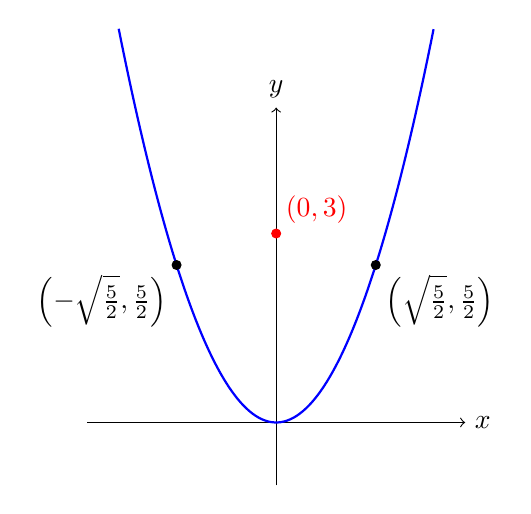
\begin{tikzpicture}[scale=0.8]
        % Ejes
        \draw[->] (-3,0) -- (3,0) node[right] {$x$};
        \draw[->] (0,-1) -- (0,5) node[above] {$y$};
        
        % Gráfica de y = x^2
        \draw[domain=-2.5:2.5, samples=100, smooth, variable=\x, blue, thick]
            plot ({\x},{\x*\x});
        
        % Punto Q (0,3)
        \filldraw[red] (0,3) circle (2pt) node[above right] {$(0,3)$};
        
        % Puntos de distancia mínima
        \filldraw[black] ({sqrt(5/2)}, {5/2}) circle (2pt) node[below right] {$\left(\sqrt{\frac{5}{2}},\frac{5}{2}\right)$};
        \filldraw[black] ({-sqrt(5/2)}, {5/2}) circle (2pt) node[below left] {$\left(-\sqrt{\frac{5}{2}},\frac{5}{2}\right)$};
    \end{tikzpicture}
    \end{center}
    
    \medskip
    
    Por lo tanto, los puntos en \( y=x^2 \) más cercanos a \( (0,3) \) son 
    \[
    \left(\sqrt{\frac{5}{2}}, \frac{5}{2}\right) \quad \text{y} \quad \left(-\sqrt{\frac{5}{2}}, \frac{5}{2}\right),
    \]
    cada uno a una distancia de \( \frac{\sqrt{11}}{2} \) unidades de \( (0,3) \).
    
    \end{solution}
    
De aquí se obtienen las raíces:
\[
a=0 \quad \text{o} \quad 2a^2-5=0 \Longrightarrow a^2=\frac{5}{2} \Longrightarrow a=\pm\sqrt{\frac{5}{2}}.
\]

Analizando la segunda derivada:
\[
\frac{d^2}{da^2}\left(a^4-5a^2+9\right)=12a^2-10.
\]
Evaluamos:
\begin{itemize}
    \item En \( a=0 \): \( 12(0)^2-10=-10<0 \) (punto de máximo).
    \item En \( a^2=\frac{5}{2} \): \( 12\left(\frac{5}{2}\right)-10=30-10=20>0 \) (mínimo).
\end{itemize}

Así, los puntos que minimizan la distancia son
\[
\left(\sqrt{\frac{5}{2}}, \frac{5}{2}\right) \quad \text{y} \quad \left(-\sqrt{\frac{5}{2}}, \frac{5}{2}\right).
\]
La distancia mínima es:
\[
d_{\min} = \sqrt{\left(\sqrt{\frac{5}{2}}\right)^2+\left(\frac{5}{2}-3\right)^2} 
= \sqrt{\frac{5}{2}+\left(-\frac{1}{2}\right)^2} 
= \sqrt{\frac{5}{2}+\frac{1}{4}}
= \sqrt{\frac{10+1}{4}} = \frac{\sqrt{11}}{2}.
\]

\medskip

\textbf{Gráfica:}

\begin{center}
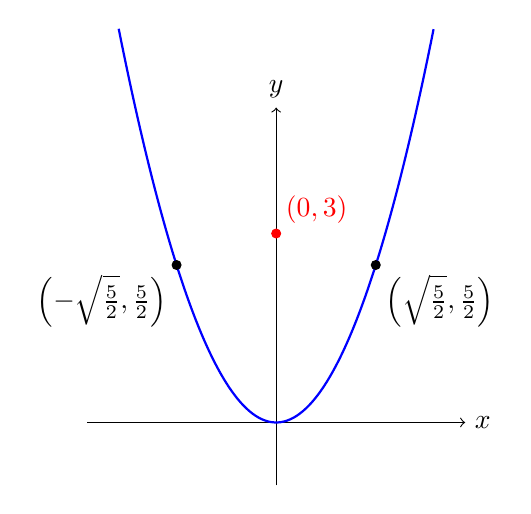
\begin{tikzpicture}[scale=0.8]
    % Ejes
    \draw[->] (-3,0) -- (3,0) node[right] {$x$};
    \draw[->] (0,-1) -- (0,5) node[above] {$y$};
    
    % Gráfica de y = x^2
    \draw[domain=-2.5:2.5, samples=100, smooth, variable=\x, blue, thick]
        plot ({\x},{\x*\x});
    
    % Punto Q (0,3)
    \filldraw[red] (0,3) circle (2pt) node[above right] {$(0,3)$};
    
    % Puntos de distancia mínima
    \filldraw[black] ({sqrt(5/2)}, {5/2}) circle (2pt) node[below right] {$\left(\sqrt{\frac{5}{2}},\frac{5}{2}\right)$};
    \filldraw[black] ({-sqrt(5/2)}, {5/2}) circle (2pt) node[below left] {$\left(-\sqrt{\frac{5}{2}},\frac{5}{2}\right)$};
\end{tikzpicture}
\end{center}

\medskip

Por lo tanto, los puntos en \( y=x^2 \) más cercanos a \( (0,3) \) son 
\[
\left(\sqrt{\frac{5}{2}}, \frac{5}{2}\right) \quad \text{y} \quad \left(-\sqrt{\frac{5}{2}}, \frac{5}{2}\right),
\]
cada uno a una distancia de \( \frac{\sqrt{11}}{2} \) unidades de \( (0,3) \).

\end{solution}

\end{document}